
\documentclass[11pt]{article}

\usepackage{amsmath}
\usepackage{amssymb}
\usepackage{graphicx}
\usepackage{booktabs}
\usepackage{hyperref}
\usepackage{geometry}
\geometry{margin=1in}

\title{The Prime Exponent Tree (PET): \\
Structural Complexity of Integer Factorization}

\author{Giancarlo Cicellyn Comneno \\
Giadaware Labs}

\date{\today}

\begin{document}

\maketitle

\begin{abstract}
We introduce the Prime Exponent Tree (PET), a recursive structural representation
of integers derived from prime factorization. Using a dataset containing all
integers up to $10^6$, we explore the structural space of integer factorizations.

Despite the large number of integers, only 78 distinct structural shapes appear
in this range. Furthermore, the distribution of these shapes is highly
concentrated: seven structures account for roughly 87\% of all integers.

We measure the structural entropy of PET shapes and observe empirically that
the complexity of integer multiplicative structure grows approximately as
$\log\log N$.
\end{abstract}

\section{Introduction}

Prime factorization reveals the multiplicative structure of integers.
However, most analyses focus on the values of primes rather than the
structural patterns formed by factorizations.

The Prime Exponent Tree (PET) represents integers as recursive trees in
which prime bases are nodes and exponents are expanded recursively as
subtrees.

This representation allows us to study the structural geometry of
integer factorizations.

\section{Prime Exponent Tree}

Let

\begin{equation}
N = \prod_i p_i^{e_i}
\end{equation}

be the prime factorization of $N$.

In the PET representation:

\begin{itemize}
\item each prime $p_i$ corresponds to a node
\item if $e_i = 1$ the node is a leaf
\item if $e_i > 1$ the exponent is represented by another PET subtree
\end{itemize}

Example:

\begin{verbatim}
12 = 2^2 * 3

•
├─2
│  •
│  └─2
└─3
\end{verbatim}

\section{Dataset}

We generated PET representations for all integers from 2 to $10^6$.

The dataset contains 999,999 integers and approximately 180MB of JSONL data.

Only

\begin{center}
78 structural shapes
\end{center}

appear within this range.

\section{Height Distribution}

\begin{center}
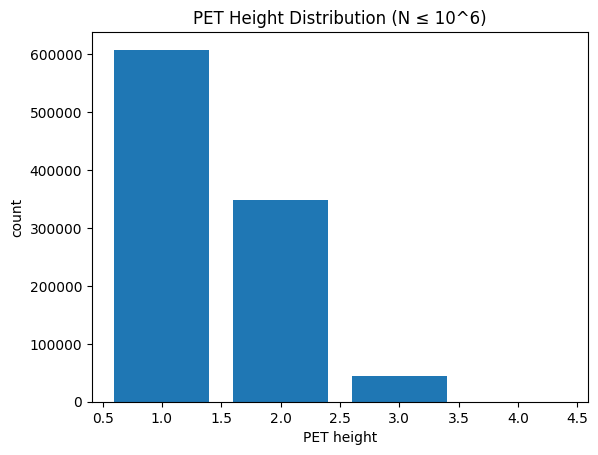
\includegraphics[width=0.7\textwidth]{figures/height_distribution.png}
\end{center}

95.6\% of integers have PET height $\le 2$.

\section{Branching Distribution}

\begin{center}
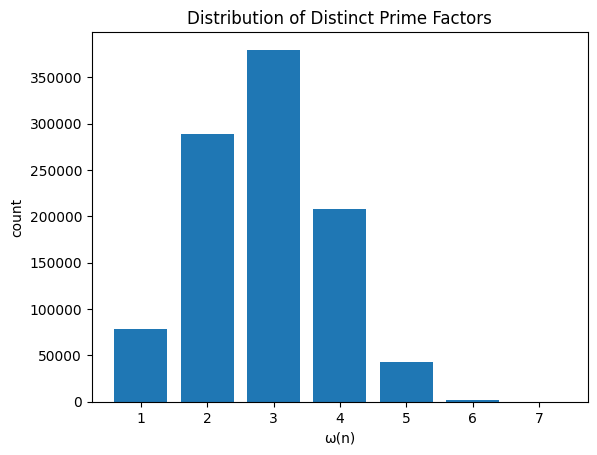
\includegraphics[width=0.7\textwidth]{figures/omega_distribution.png}
\end{center}

The branching factor corresponds to $\omega(n)$,
the number of distinct prime factors.

\section{Structural Entropy}

The entropy of PET shapes is defined as

\begin{equation}
H = -\sum_i p_i \log p_i.
\end{equation}

For integers $\le 10^6$ we obtain

\begin{center}
$H \approx 2.35$
\end{center}

with maximum possible entropy

\begin{center}
$\log 78 \approx 4.36$.
\end{center}

\section{Entropy Growth}

\begin{center}
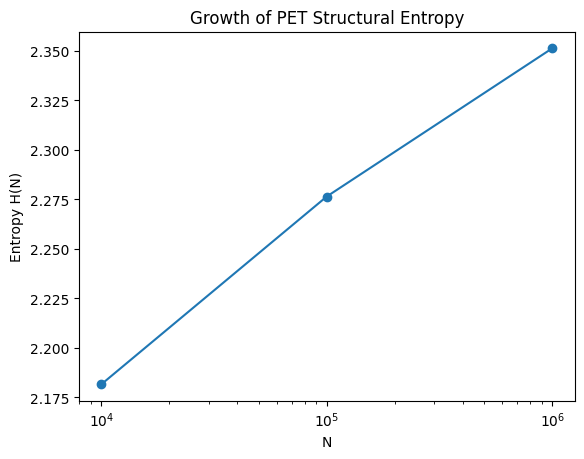
\includegraphics[width=0.7\textwidth]{figures/entropy_growth.png}
\end{center}

Empirically we observe

\begin{equation}
H(N) \sim \log\log N.
\end{equation}

\section{Conclusion}

The Prime Exponent Tree representation reveals that the multiplicative
structure of integers occupies a remarkably small combinatorial space.

Even for one million integers, only a few dozen structural shapes appear,
and the effective complexity of this structure grows extremely slowly.

\end{document}
